\documentclass[11pt]{article}
\usepackage[margin=1in]{geometry}
\usepackage{graphicx}
\usepackage{booktabs}
\usepackage{amsmath,amssymb}
\usepackage{xcolor}
\usepackage[hidelinks]{hyperref}
\usepackage{caption}
\usepackage{float}
\usepackage{enumitem}
\definecolor{codecol}{RGB}{160,60,90}
\newcommand{\code}[1]{\texttt{\textcolor{codecol}{#1}}}
\setlength{\parskip}{0.5em}\setlength{\parindent}{0pt}
\captionsetup{font=small,labelfont=bf}
\graphicspath{{figures/}}

\title{\vspace{-1.5em}\textbf{SpectraForge}\\[0.2em]
{\large A Physics-Grounded Synthetic Testbed for 4D Fluorescence Hyperspectral Imaging,\\
and What It Taught Us About Autoencoder Band Selection}}
\author{Narek Meloyan \and Narine Sarvazyan}
\date{Internal review draft, July 2026}

\begin{document}
\maketitle
\vspace{-1em}

\begin{abstract}
\noindent This is an internal, story-first write-up for supervisors and collaborators. It
has two subjects. The first, and the one we care about most, is \textbf{SpectraForge}: a
physics-grounded generator that turns the equations of fluorescence into synthetic 4D
excitation-emission cubes with \emph{perfect ground truth}, built so that the loudest bands
are deliberately not the informative ones. We explain what it does, the photophysics and the
math behind it, and why it is a tool the 4D fluorescence imaging community can use. The second
subject is what we \emph{learned} by running our autoencoder (AE) band-selection idea on it:
a debugging story that took a published model from chance to competitive, a
significance-tested verdict on where a learned selector genuinely helps (and where classical
methods already suffice), and one clean structural result. We keep the account honest, because
the value of the benchmark is precisely that it does not let us fool ourselves.
\end{abstract}

\section*{0. The one-page version}
\begin{itemize}[leftmargin=1.4em,itemsep=0.2em]
\item \textbf{SpectraForge} renders 4D fluorescence cubes (excitation $\times$ emission $\times$
height $\times$ width) from a parametric fluorophore model obeying Kasha, Vavilov,
Franck--Condon and the Stokes shift, with optional inner-filter, reabsorption, FRET, scatter,
noise, and instrument clutter. Every cube ships with ground truth, and scenes are constructed
so that \textbf{band variance is decoupled from class informativeness} (measured correlation
$\approx -0.1$). That single property is what makes it an \emph{honest} benchmark instead of a
trivial one.
\item It fills a real gap: labeled real 4D fluorescence data is scarce and has no ground truth,
so you cannot tell a selector which bands it \emph{should} have found. SpectraForge can, on
demand, at controllable difficulty, with real dye spectra importable from FPbase and an
interactive painting GUI.
\item Using it, we took a published perturbation-CAE selector \textbf{from chance
(macro-F1 $\approx 0.33$) to competitive}, by fixing four real trainer bugs, a misleading
metric, and one architectural flaw (an emission-axis ``band collapse'').
\item The honest, significance-tested verdict: the AE+perturbation selector \textbf{matches}
the strongest classical blind method (PCA loadings) on realistic data, \textbf{significantly
beats} it on nonlinear reabsorption ($0.449$ vs $0.431$, $95\%$ CI excludes $0$), and
\textbf{ties} it on FRET. It is a sound, fully-unsupervised selector, not a dominant one.
\item The two lessons that generalize: (i) \textbf{band selection is not classification}
(``informative $\Rightarrow$ has variance $\Rightarrow$ PCA finds it''); and (ii) the one place
a convolutional model is \emph{structurally necessary} is \textbf{spatial-texture}
discrimination, where per-pixel selection is provably blind.
\end{itemize}

\section{The problem, and why we built a simulator}
A multi-excitation hyperspectral cube illuminates a sample at several excitation wavelengths and,
for each, records an emission spectrum across many bands. Every pixel therefore carries an
\textbf{excitation--emission matrix} (EEM), and a whole scene is a four-dimensional array over
(excitation, emission, $y$, $x$). This is the modality behind a lot of biomedical and material
fluorescence imaging, because different fluorophores, tissue states, or species separate cleanly
in the joint excitation--emission domain. The catch is dimensionality: the per-pixel feature vector
(excitations $\times$ emission bands) is large and mostly redundant, and only a small subset of
bands actually distinguishes the classes. \textbf{Band selection} is the task of finding that
subset, so a cheaper instrument can acquire only the informative bands, or a classifier can run on
a compact feature set.

To develop a band selector you need to know which bands are truly informative, so you can measure
whether the selector found them. On real data you never know this. And when people build synthetic
data, they almost always make it \emph{too kind}: the discriminative dyes are also the brightest, so
``pick the loudest bands'' wins and every method looks good. That tells you nothing. What we needed
was synthetic data that is (a) physically faithful, (b) equipped with ground truth, and (c)
deliberately hard in the way real fluorescence is hard: where the signal you want is \emph{not} the
loudest thing in the cube. That is SpectraForge.

\section{SpectraForge: turning photophysics into an honest benchmark}

\subsection{The physics, briefly}
A fluorophore absorbs a photon (ground state $S_0 \to S_1, S_2, \dots$, femtoseconds), tumbles
down non-radiatively to the lowest vibrational level of $S_1$ (picoseconds), and only then emits
(nanoseconds). Four textbook consequences shape the EEM, and SpectraForge encodes each:

\begin{itemize}[leftmargin=1.4em,itemsep=0.15em]
\item \textbf{Kasha's rule} --- emission leaves from that lowest $S_1$ level \emph{regardless of how
you excited it}. So the emission \emph{shape} does not depend on excitation wavelength, and the EEM
factorizes into an excitation profile $\times$ an emission profile $\times$ a concentration. This
separability is the basis of PARAFAC, and, as we will see, it \emph{is} Kasha's rule written as
algebra.
\item \textbf{Vavilov's rule} --- the quantum yield is, to first order, independent of excitation
wavelength. Exciting at $350$ or $480\,$nm changes \emph{how many} molecules emit, not \emph{what
colour}: only the amplitude scales.
\item \textbf{Franck--Condon} --- electronic transitions are vertical on the nuclear-coordinate
diagram, which sets the broadened, roughly mirror-image band envelopes and an optional vibronic
shoulder about $1300\,\mathrm{cm}^{-1}$ to the red (the thing that gives a dye its characteristic
shape).
\item \textbf{Stokes shift} --- because emission ends on excited vibrational levels of $S_0$, the
photon is red-shifted from absorption, separating the emission peak from the Rayleigh line.
\end{itemize}

\subsection{The forward model (the actual equations)}
Each fluorophore $k$ is a small parametric object: a peak-normalized Gaussian excitation profile
$a_k(\lambda_\mathrm{ex})$, an area-normalized (optionally red-tailed, vibronic) emission profile
$e_k(\lambda_\mathrm{em})$, an extinction $\varepsilon_k$, a quantum yield $\Phi_k$ (its brightness
is the product $\varepsilon_k\Phi_k$), and a per-pixel concentration map $c_k(x,y)$. A single
fluorophore's contribution to the cube is
\begin{equation}
S_k(x,y,\lambda_\mathrm{ex},\lambda_\mathrm{em})
= \underbrace{c_k(x,y)}_{\text{amount}}\;
\underbrace{\varepsilon_k\Phi_k}_{\text{brightness}}\;
\underbrace{a_k(\lambda_\mathrm{ex})}_{\text{excitation}}\;
\underbrace{e_k(\lambda_\mathrm{em})}_{\text{emission}},
\end{equation}
and the rendered cube is the dilute linear superposition (the linear mixing model, with a global
lamp/exposure/power gain $g$):
\begin{equation}
F(x,y,\lambda_\mathrm{ex},\lambda_\mathrm{em}) = g\sum_k S_k .
\end{equation}
With every optional effect switched off this model is \emph{exactly linear}, and the code checks the
invariant $\mathrm{render}(A+B) = \mathrm{render}(A) + \mathrm{render}(B)$. The excitation and emission
profiles are Gaussian,
\begin{equation}
a_k(\lambda)=\exp\!\Big(\!-\tfrac{(\lambda-\lambda^{\mathrm{ex}}_k)^2}{2\sigma_k^2}\Big),
\qquad
e_k(\lambda)=\tfrac{1}{Z_k}\exp\!\Big(\!-\tfrac{(\lambda-\lambda^{\mathrm{em}}_k)^2}{2\tau_k^2}\Big),
\end{equation}
with widths $\sigma_k,\tau_k=\mathrm{FWHM}/(2\sqrt{2\ln 2})$; $a_k$ is peak-normalized and $e_k$
area-normalized ($Z_k$ is the normalizer), and an optional red skew plus a vibronic shoulder
$\sim\!1300\,\mathrm{cm}^{-1}$ to the red refine the emission shape. A fluorophore's brightness is the
product $\varepsilon_k\Phi_k$, with quantum yield $\Phi_k=k_r/(k_r+k_{nr})$ (radiative over total
decay). Everything hard about the
benchmark is then added back in physically faithful, opt-in increments. Figure~\ref{fig:fluoro}
shows the dye model: a few dim, overlapping discriminative dyes and a couple of bright, useless
nuisances.

\begin{figure}[H]\centering
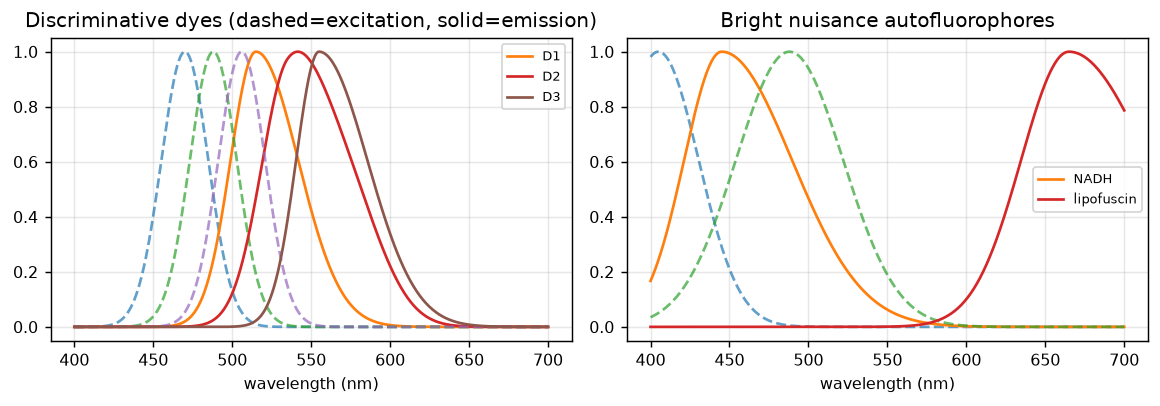
\includegraphics[width=\linewidth]{fig_fluorophores.png}
\caption{The parametric fluorophore model. Left: three discriminative dyes (dashed excitation,
solid emission), modest brightness, overlapping emission, distinct excitation. Right: two bright
nuisance autofluorophores (NADH-like, lipofuscin-like) that dominate band variance while carrying
no class information.}
\label{fig:fluoro}
\end{figure}

\subsection{The one design decision that matters: variance $\ne$ informativeness}
Here is the heart of it. SpectraForge paints \emph{discriminative} dyes with smooth random
concentration fields whose per-pixel argmax \emph{is the class label}; these dyes are deliberately
dim and spectrally overlapping, so their discriminative content lives in low-variance band
\emph{shape}. Then it paints independent \emph{nuisance} dyes that are bright and spatially varying
but class-irrelevant. Real physics decouples variance from class in four independent ways, and the
generator reproduces all of them:
\begin{enumerate}[leftmargin=1.6em,itemsep=0.1em]
\item \emph{high variance, zero information} --- Rayleigh and Raman scatter ridges;
\item \emph{high variance, class-irrelevant} --- bright autofluorescence nuisances with their own
spatial fields;
\item \emph{inflated variance} --- shot noise makes bright (possibly redundant) bands look important;
\item \emph{low-variance signal} --- the discriminating information sits in dim dyes or in the subtle
shape difference between overlapping bands.
\end{enumerate}
The consequence is measurable and is the property that makes the benchmark honest: on a confounded
scene the correlation between per-band variance and per-band discriminability is $\approx -0.1$,
versus strongly positive on naive clean data (Figure~\ref{fig:scene}). A ``pick the loudest bands''
strategy therefore \emph{fails by construction}, which is exactly what we want, because that is what
real fluorescence does.

\begin{figure}[H]\centering
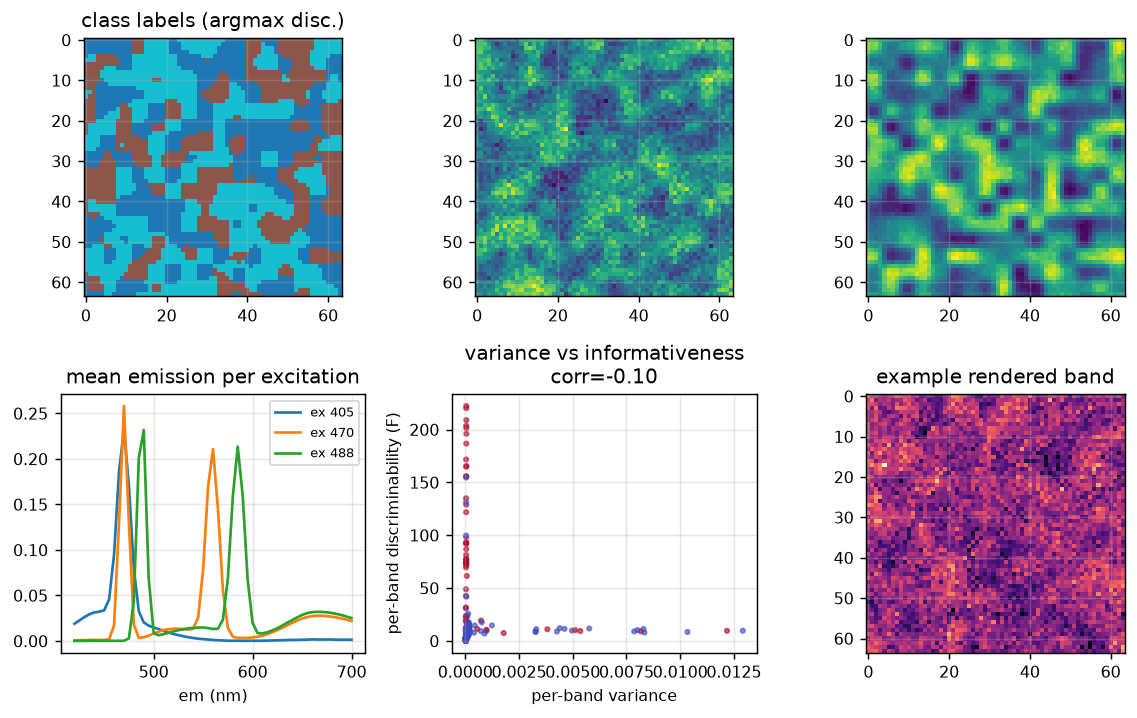
\includegraphics[width=\linewidth]{fig_scene.png}
\caption{The forward model and the variance-versus-informativeness property. Top: class labels and
example rendered bands (a discriminative-dye band, a Rayleigh scatter band, a nuisance band).
Bottom: mean emission per excitation; then the scatter of per-band variance against per-band
discriminability, whose near-zero (slightly negative) correlation is printed --- the loudest bands
are not the informative ones; then an example rendered band.}
\label{fig:scene}
\end{figure}

\subsection{Making it realistic: scatter, noise, nonlinearity, clutter}
On top of the clean cube the generator adds \textbf{Rayleigh scatter} (a bright line at
$\lambda_\mathrm{em}=\lambda_\mathrm{ex}$ plus a grating ghost at $2\lambda_\mathrm{ex}$) and a
\textbf{water Raman} line at a fixed wavenumber offset ($\approx 3400\,\mathrm{cm}^{-1}$), each
scaled by a per-pixel turbidity field, then \textbf{Poisson shot noise} and Gaussian
\textbf{read noise}. Three optional effects break linearity in concentration, which is where a
nonlinear method \emph{could} in principle beat a linear one:
\begin{itemize}[leftmargin=1.4em,itemsep=0.1em]
\item \textbf{Primary inner filter}: local signal attenuated by $\exp(-s\,A_\mathrm{ex})$.
\item \textbf{Reabsorption} (secondary inner filter): emission attenuated by
$\exp(-s\,A_\mathrm{em}(\lambda))$; because absorption overlaps the blue edge of emission, this
\emph{reshapes the band} and apparent-red-shifts the peak as a function of concentration, relocating
discriminative information into band shape (Figure~\ref{fig:reab}).
\item \textbf{FRET}: for a donor--acceptor pair, a saturating fraction $E = k c_A/(1+k c_A)$ of donor
energy transfers to the acceptor; the donor is quenched and the acceptor sensitized, which encodes
dye \emph{co-localization} in a band ratio --- a genuinely nonlinear (product/XOR-like) class signal.
\end{itemize}
Written out, the optional physics is
\begin{align}
\text{inner filter:}\quad & F = F_{\mathrm{obs}}\,10^{-(A_{\mathrm{ex}}+A_{\mathrm{em}})/2},\\
\text{reabsorption:}\quad & A_{\mathrm{em}}(\lambda)=\textstyle\sum_k \varepsilon_k c_k\,\alpha_k(\lambda),\\
\text{Raman line:}\quad & 1/\lambda_R = 1/\lambda_{\mathrm{ex}}-\Delta\bar\nu,\ \ \Delta\bar\nu\approx 3400\,\mathrm{cm}^{-1},\\
\text{FRET:}\quad & E = k\,c_A/(1+k\,c_A),
\end{align}
with Rayleigh at $\lambda_{\mathrm{em}}=\lambda_{\mathrm{ex}}$ (and a ghost at $2\lambda_{\mathrm{ex}}$); the
primary and secondary inner filter are realized as multiplicative factors $e^{-sA_{\mathrm{ex}}}$ and
$e^{-sA_{\mathrm{em}}(\lambda)}$; FRET scales the donor by $(1-E)$ and adds
$E\cdot(\text{absorbed donor})\cdot\Phi_A$ to the acceptor; and each pixel receives Poisson shot noise
(variance $=$ mean) plus Gaussian read noise.
Finally, \textbf{fixed-pattern clutter} injects many independent class-irrelevant low-rank spatial
fields onto random band subsets (the analogue of illumination/detector artifacts). Clutter is
high-variance and class-irrelevant, and it turns out to be the dominant real-instrument confound
(Figure~\ref{fig:clutter}).

\begin{figure}[H]\centering
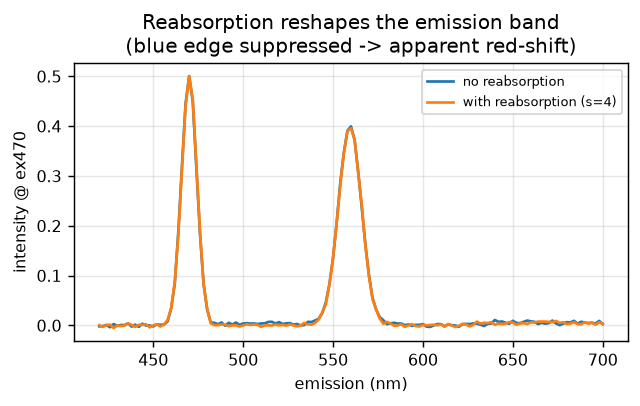
\includegraphics[width=0.72\linewidth]{fig_reabsorption.png}
\caption{Reabsorption reshapes the band. A bright pixel's emission at ex470 with and without
reabsorption (strength 4): the blue edge is suppressed, producing an apparent red-shift ---
a concentration-dependent, nonlinear reshaping that relocates discriminative information into shape.}
\label{fig:reab}
\end{figure}

\begin{figure}[H]\centering
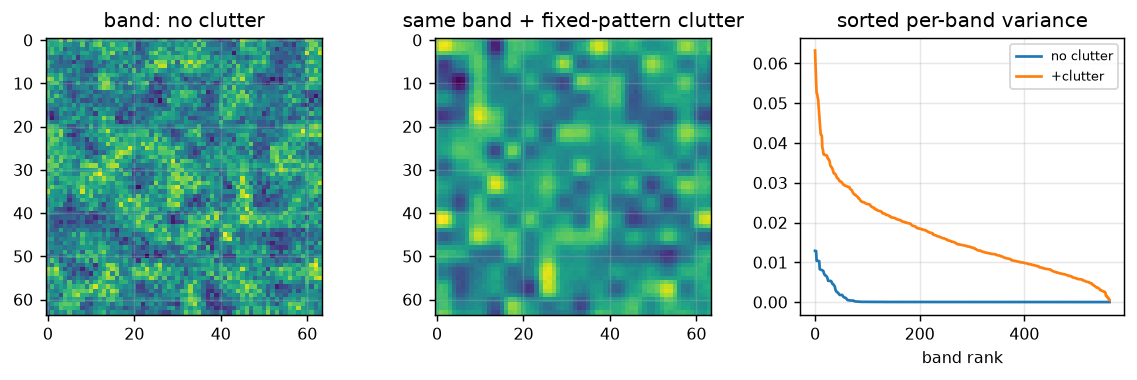
\includegraphics[width=\linewidth]{fig_clutter.png}
\caption{Fixed-pattern clutter. Left/middle: the same band before and after injecting 36
class-irrelevant low-rank spatial clutter modes. Right: sorted per-band variance --- clutter raises
the variance of many bands without adding any class information, which is exactly why
variance- and reconstruction-based selection collapses to chance.}
\label{fig:clutter}
\end{figure}

\subsection{Building a scene: what the user does}
SpectraForge is not only equations; it is an interactive application, so building data feels like
working in an image editor rather than writing a simulator (Figs.~\ref{fig:gui-lib}--\ref{fig:gui}):
\begin{enumerate}[leftmargin=1.6em,itemsep=0.1em]
\item \textbf{Pick or define the chemicals.} Choose fluorophores from a built-in library (or import
real measured spectra from FPbase), or define a new dye by its excitation and emission peaks, band
widths, quantum yield, and extinction (Fig.~\ref{fig:gui-lib}).
\item \textbf{Mix them into materials.} A material is a recipe, a set of fluorophore concentrations
(for example collagen with a little NADH), previewed live as a spectrum.
\item \textbf{Paint the sample.} Draw each material onto the canvas with a brush, rectangle, or
circle; the per-pixel amount you paint becomes its concentration map.
\item \textbf{Organize in layers.} Stack materials as layers you can toggle and reorder, exactly like
an image editor; the per-pixel dominant discriminative material sets the class label.
\item \textbf{Acquire, render, select, validate.} Set the excitation wavelengths and emission grid,
render the 4D cube, run a band selector, and press one button to score the selection against the
ground truth (Fig.~\ref{fig:gui}).
\end{enumerate}
The whole loop, from picking chemicals to a scored band selection, runs in one window, which is what
makes SpectraForge usable as a design tool for a real experiment and not only as a benchmark.

\begin{figure}[H]\centering
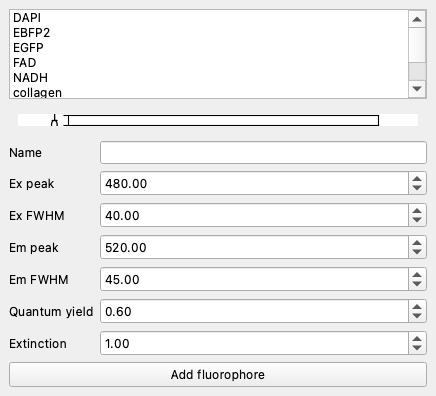
\includegraphics[width=0.60\linewidth]{fig_gui_library.png}
\caption{Picking and defining chemicals. The fluorophore library (top list) and the editor for a
fluorophore's photophysical parameters: excitation and emission peak and width, quantum yield, and
extinction. New dyes are added here, or imported from FPbase.}
\label{fig:gui-lib}
\end{figure}

\begin{figure}[H]\centering
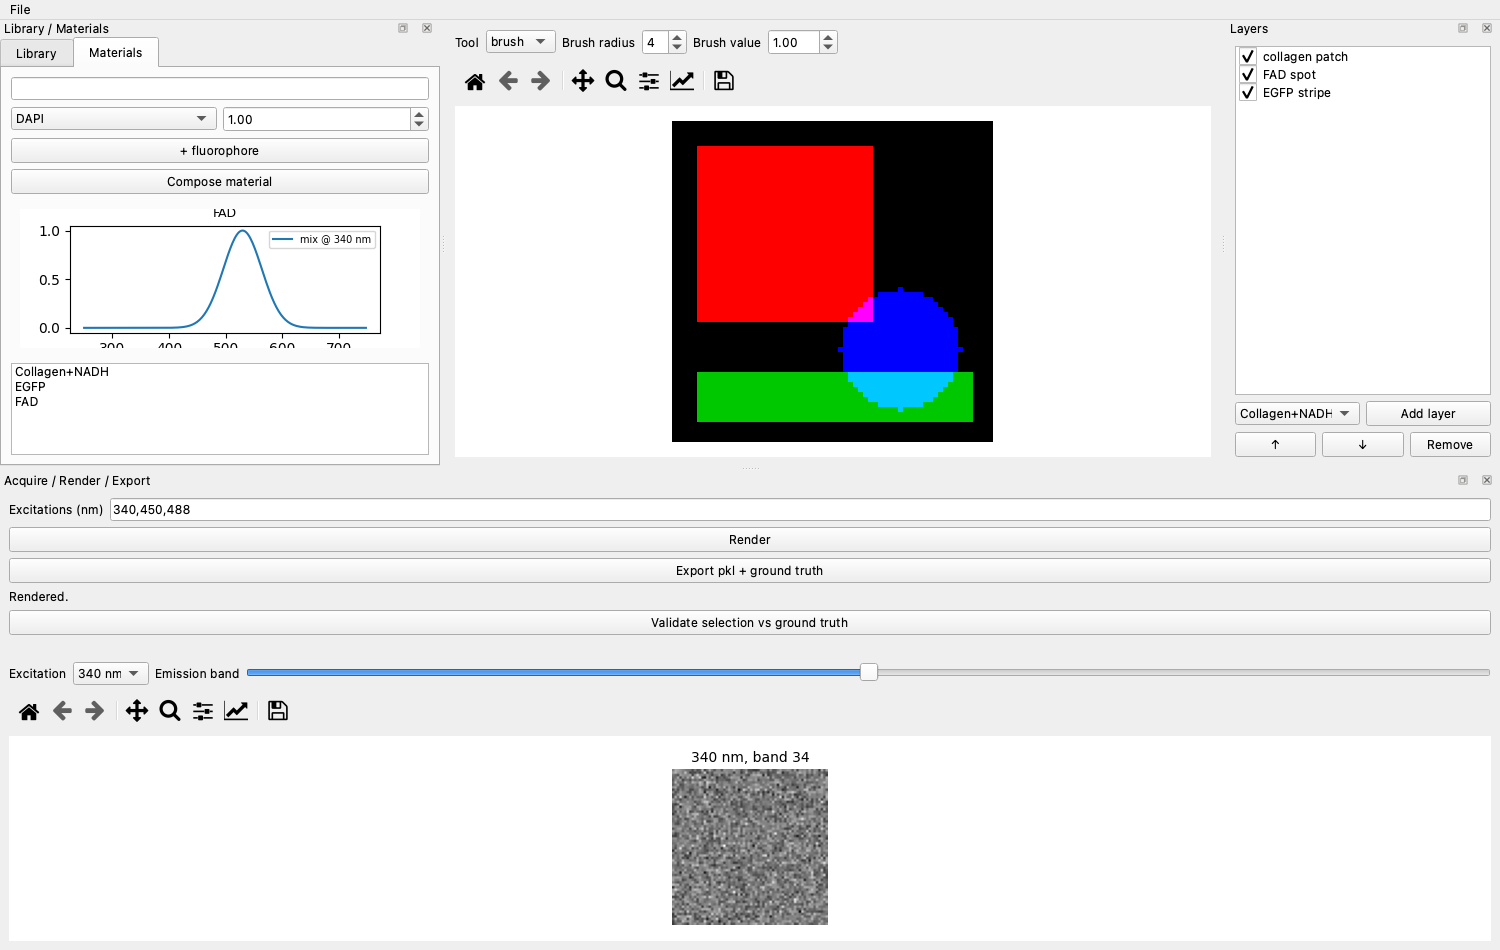
\includegraphics[width=\linewidth]{fig_gui.png}
\caption{The SpectraForge workbench: one window for the whole workflow. Left: materials (fluorophore
recipes) with a live spectrum preview. Centre: the painted canvas (a collagen+NADH patch, an FAD
spot, an EGFP stripe), whose colours are the class labels. Right: the layer stack. Bottom: acquire,
render, and validate, here previewing a rendered emission band at 340\,nm with the one-click
``Validate selection vs ground truth''.}
\label{fig:gui}
\end{figure}

\subsection{Regimes, ground truth, and how you actually use it}
Dialing these knobs spans a ladder of regimes from one \code{build\_dataset(\dots)} call:
\textbf{clean} (variance $\approx$ informativeness), \textbf{realistic} (strong nuisances, scatter,
noise), \textbf{clutter}, \textbf{nonlinear} (reabsorption or FRET/XOR), and \textbf{spatial-texture}
(class carried by spatial pattern with identical per-pixel spectra). Every render returns a
\code{GroundTruth} sidecar with concentration maps, clean cubes, and each dye's true emission peak,
which enables both broad information-retention metrics and a \emph{tight} \code{peak\_recovery}
metric (did a selected band land within a tolerance of a true peak? a random selector scores
$\approx 0.33$). A companion script re-runs every simulation and writes the exact parameters, so
figures and numbers are reproducible. The parametric dyes can be swapped for \emph{real measured
spectra imported from FPbase}, and there is an interactive PyQt ``Forge'' workbench where you paint
concentration maps, render, and press a button to validate a selection against ground truth.

\subsection{Why this is worth having (the point of the tool)}
The community lacks an open, physically faithful source of 4D fluorescence cubes with ground truth
and controllable difficulty. SpectraForge is that. It lets you (i) benchmark any band-selection,
dimensionality-reduction, or classification method against a known answer; (ii) dial difficulty in
physically meaningful increments (add scatter, add nuisances, add clutter, turn on nonlinear
physics) rather than by fiddling opaque noise levels; and (iii) do all of this while preserving the
exact-linear invariant when confounds are off, so you always know what you are testing. And, as the
rest of this document shows, it does the thing a good benchmark is supposed to do: it caught a real
methodological failure of ours that raw training loss had hidden completely.

\section{What we learned running our CAE on it}

\subsection{The idea, and the crisis}
The method we wanted to validate is \textbf{autoencoder + latent-perturbation} selection: train an
AE to reconstruct the cube; perturb each latent dimension and measure how strongly each input band's
reconstruction responds; accumulate those per-band sensitivities into an influence score; keep the
top-$k$ (with a diversity constraint). Concretely, for a per-pixel latent code $z$ the per-band
influence accumulates the reconstruction change under a perturbation $\delta$ of each retained latent
coordinate $j$,
\begin{equation}
I_b=\sum_{j}\sum_{\delta} w_j\;\frac{1}{NP}\sum_{n=1}^{N}\sum_{p=1}^{P}
\big|[\,D(z_n+\delta e_j)-D(z_n)\,]_{p,b}\big|,
\end{equation}
where $D$ is the decoder, $N$ the number of samples, $P$ the pixels, $e_j$ the $j$-th unit vector, and
$w_j$ a per-coordinate weight; bands are chosen greedily from $I_b$ with a redundancy penalty. It is
appealing because it is fully unsupervised yet, being
nonlinear, could in principle catch structure PCA cannot. Run on SpectraForge and scored honestly,
the published convolutional version \textbf{selected at chance} (macro-F1 $\approx 0.33$ on a 3-class
scene) and reconstructed almost nothing. Either the pipeline was corrupting pixels, the training was
broken, or the architecture could not represent the data. We were warned explicitly that ``the loss
alone can be deceiving'' --- and it was.

\subsection{Four real bugs}
A pipeline-integrity check showed the chunking/batching was lossless to $\sim 10^{-8}$, so the
failure was in the model or training. Inspecting the trainer turned up \textbf{four genuine bugs},
each independently able to cripple a run:
\begin{enumerate}[leftmargin=1.6em,itemsep=0.1em]
\item a \code{ReduceLROnPlateau(verbose=\dots)} call that \emph{crashes} on modern PyTorch;
\item an \code{UnboundLocalError} when the loss never improves or is NaN (the best-model path is
never assigned, then loaded);
\item a \code{0.0 * NaN = NaN} sparsity term that poisoned the loss \emph{even when its weight was
zero}, so every non-sigmoid-latent run silently trained on NaN and learned nothing;
\item a \code{scheduler\_patience = 5} default that halves the learning rate after five stalled
epochs, freezing the model near initialization.
\end{enumerate}
The published default config is byte-identical after the fixes; we only removed the failure modes.

\subsection{The metric was lying too}
Our own first verdict --- ``$R^2 < 0$, reconstructs nothing'' --- used per-band-averaged $R^2$, which
is dominated by the $\sim 40$ of $57$ off-peak noise bands that \emph{no} model can reconstruct.
Switching to signal-band correlation, and measuring the achievable ceiling with a per-pixel MLP
control ($\approx 0.49$, not $1.0$), reframed every later comparison. Lesson: on sparse spectra,
average reconstruction error is not a proxy for whether the model captured the signal.

\subsection{The architectural flaw: the band collapse}
With the bugs fixed and the honest metric in hand, the published CAE \emph{still} reconstructed
nothing on multi-fluorophore data (signal correlation $\approx 0.001$) yet worked on a single-dye
scene ($\approx 0.34$). That dissociation localized the fault exactly: the emission-axis
\code{adaptive\_avg\_pool3d} \textbf{averages over emission}, so it cannot represent different spatial
patterns at different emission bands --- which is precisely what distinguishes multiple fluorophores.
Removing the collapse, and nothing else about the idea, raised reconstruction about $100\times$
($0.001 \to 0.104$) and took selection \textbf{from chance $0.331$ to $0.414$, about $85\%$ of the
labels-using oracle ($0.486$)}. So the answer to ``is it a bug or the architecture?'' was
\emph{both}.

\subsection{Recovery, and a swarm}
A repeatedly-confirmed finding shaped the search: \textbf{reconstruction fidelity is
anti-correlated with selection quality} --- the selection knobs matter more than the last bit of
reconstruction. Tuning the perturbation (PCA-ranked latent dims, standard-deviation perturbation,
$\sim 80$ accumulated dims) lifted selection to $0.438$ ($90\%$ of oracle); a per-pixel
collapse-\emph{bottleneck} conv-AE reached $\mathbf{0.473 \pm 0.018}$ on clean, matching PCA loadings
($\approx 0.48$, $97\%$ of oracle). A flexible-architecture swarm over depth, width, latent size,
activation, masking/denoising, and MLP-vs-1D-conv backbones found that masking/denoising is the
dominant lever on clean data ($0.50$--$0.51$, exceeding PCA), and a conv-over-bands backbone at
modest depth is best on realistic data ($0.464$); depth and width beyond that gave nothing,
confirming a ceiling rather than a tuning shortfall.

\subsection{The honest, significance-tested verdict}
To keep ourselves honest we ran a full battery: five metric families over eight selectors, several
regimes, six seeds, with bootstrap confidence intervals and, crucially, a \textbf{random} baseline
and the \textbf{full spectrum} as controls. The headline comparison of the best AE against the
strongest classical blind selector (PCA loadings) is Table~\ref{tab:battery}.

\begin{table}[H]\centering
\caption{Significance battery: AE (best of family) vs PCA loadings, best-of-panel macro-F1, six
seeds. Positive margin favours the AE.}
\label{tab:battery}
\small
\begin{tabular}{@{}lcccc@{}}
\toprule
regime & AE & PCA-load & margin & 95\% CI \\
\midrule
clean & $0.590$ & $\mathbf{0.635}$ & $-0.046$ & $[-0.079,-0.019]$ \\
realistic & $0.527$ & $0.531$ & $-0.004$ & tie \\
reabsorption & $\mathbf{0.449}$ & $0.431$ & $+0.018$ & $[+0.001,+0.029]$ \\
FRET & $0.635$ & $0.642$ & $-0.007$ & tie \\
\bottomrule
\end{tabular}
\end{table}

Read plainly: PCA loadings is the strongest blind selector overall; the AE is \textbf{competitive,
not dominant}. It ties on realistic and FRET, it \emph{significantly} beats PCA on nonlinear
reabsorption (the confidence interval excludes zero, Cohen $d \approx 0.94$), and PCA wins on clean,
low-noise data where the informative bands are also the loudest. The AE's clean advantage seen in the
swarm is real but \textbf{noise-dependent} --- its denoising only helps when there is noise to remove.

\subsection{Trying to beat PCA ``by far'': the nonlinear tests}
An AE \emph{should} win where the structure is nonlinear. We tested this directly. Under
physically-correct reabsorption, with an evaluation that credits nonlinear shape (a classifier panel
and a nonlinear-only ``gap'' metric), the AE's subset carries nonlinear-only information ($+0.030$)
that PCA's does not ($-0.021$), and the margin crosses from negative to positive as the regime
becomes more nonlinear --- the direction of the hypothesis is confirmed. But the margin is small
($\le\!\sim\!0.03$) and did not reproduce at three independent seeds, so ``by far more'' is not
supported on this data class. The strongest honest nonlinear regime is FRET on an XOR co-localization
scene, where even a marginal mutual-information oracle fails (XOR is invisible per band). There the
AE and PCA are \textbf{tied} ($0.633$ vs $0.641$, within noise), and, tellingly, the AE's
nonlinear-only gap ($+0.092$) \emph{equals} PCA's ($+0.091$). It \emph{captures} the nonlinear
structure; it just does not \emph{select} better. The reason is the single most useful thing we
learned:

\begin{quote}
\textbf{Band selection is not classification.} Informative $\Rightarrow$ has variance $\Rightarrow$
PCA selects it. The discriminative bands carry concentration-driven variance, so a linear selector
finds them; the nonlinearity (XOR, a FRET ratio) is then resolved by the \emph{downstream}
classifier, not by the selector. A nonlinear classification task does not imply a nonlinear
selection task, so the AE's manifold advantage buys nothing extra at the selection step.
\end{quote}

\subsection{Where the benchmark says to stop}
Because we always ran the two controls, SpectraForge also told us where unsupervised selection stops
helping (Figure~\ref{fig:results}). Under realistic fixed-pattern clutter, \textbf{blind selection
(AE and PCA alike) does not beat a random subset} --- only label-aware selection does --- because
clutter is high-variance but class-irrelevant, so every variance-driven criterion ranks clutter bands
about randomly with respect to class. Across label budgets, \textbf{selection never beats the full
spectrum}: its value is compression, not accuracy (both blind selectors reach $\sim 95\%$ of full at
a large budget, while labels compress about $2.7\times$ better). And both blind selectors are
\textbf{unstable} band by band (Jaccard $\approx 0.1$--$0.2$), which argues for selecting spectral
regions or consensus sets rather than exact bands. These are findings of the benchmark, and they are
useful: they tell a practitioner when to bother selecting bands at all.

\begin{figure}[H]\centering
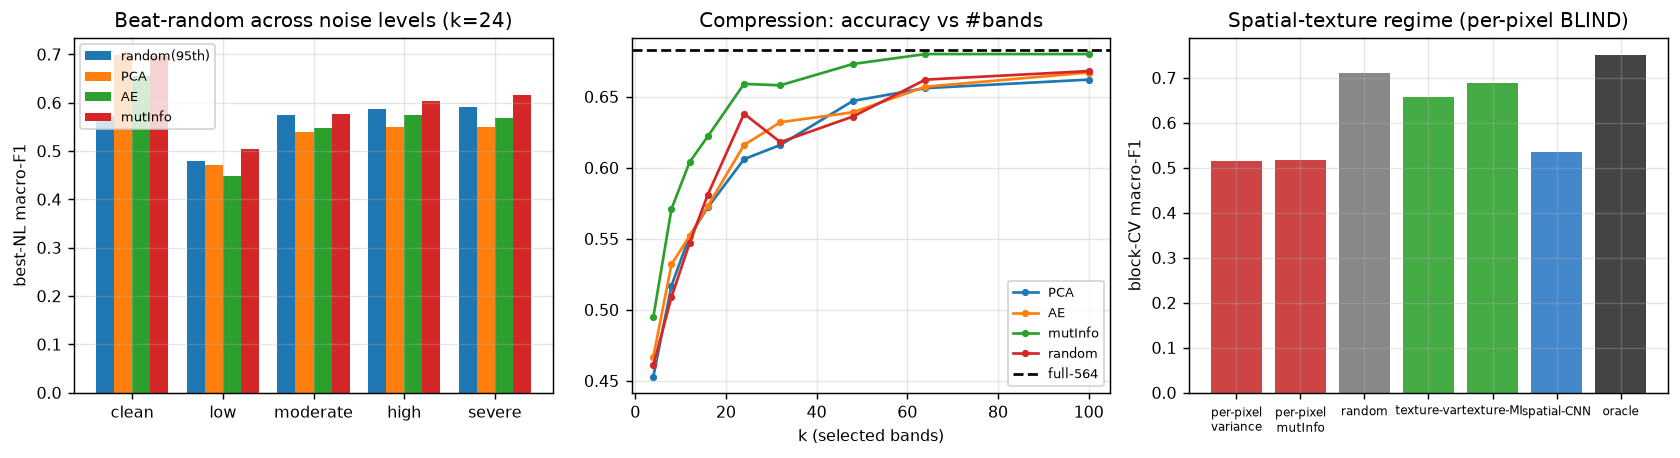
\includegraphics[width=\linewidth]{fig_results.png}
\caption{What the controls reveal. Left: beat-random across five noise levels --- blind PCA/AE beat
the random $95$th percentile only on clean data; under any clutter only supervised mutual information
does. Middle: the compression curve --- AE tracks PCA at every budget, both reaching $\sim 95\%$ of
full, while labels compress $\sim 2.7\times$ better. Right: the spatial-texture regime under honest
block cross-validation --- per-pixel selectors are the \emph{worst} (below random), while a spatial
model and the oracle succeed.}
\label{fig:results}
\end{figure}

\subsection{The one clean structural win}
There is exactly one regime where the convolutional idea is \emph{structurally necessary}. When the
class is carried by \textbf{spatial texture}, so every class has the same per-pixel spectrum,
per-pixel band selection is \textbf{provably blind}: under honest spatial-block cross-validation the
per-pixel selectors are the worst ($0.52$--$0.55$, below the random $0.674$), while a spatial model
with the discriminative bands reaches the oracle ($0.78$). This vindicates the original
spatial-CAE intuition --- but for \emph{spatial classification}, not for per-pixel spectral band
selection.

\section{What it all means}
Three mechanisms explain every result above.
\begin{enumerate}[leftmargin=1.6em,itemsep=0.1em]
\item \textbf{Selection $\ne$ classification.} The AE's nonlinearity helps a classifier, not the
choice of bands.
\item \textbf{Unsupervised $\equiv$ variance.} Reconstruction, variance, and PCA loadings all rank by
variance, which under clutter or nuisances is decoupled from class --- so they behave like random.
\item \textbf{Extractable $\Leftrightarrow$ variance-prominent.} A band strong enough to be useful is
high-variance (simple methods find it); a band that is not variance-prominent is too weak to extract.
There is no gap for a learned \emph{selector} to fill --- except genuinely spatial information, which
is invisible to per-pixel methods.
\end{enumerate}

\section{Recommendations}
\begin{itemize}[leftmargin=1.4em,itemsep=0.1em]
\item For per-pixel band selection on realistic data, use \textbf{supervised} selection (marginal
mutual information for clutter/linear structure, random-forest importance for nonlinear), and
\textbf{always} benchmark against random and full-data. If a method cannot beat a random subset, it
adds nothing.
\item Treat band selection as a \textbf{compression} tool. If you have the labels and the budget, keep
the full spectrum.
\item Select \textbf{spectral regions or consensus sets}, not exact bands --- no selector is stable
under clutter.
\item Use a \textbf{convolutional/spatial} model where discrimination has spatial structure; that is
its real, provable value.
\item Validate on \textbf{real data} with the same controls. This is the open gate.
\end{itemize}

\section{Open gate: real data}
The decisive next step is to run the winning configuration on the actual Lichens and Collagen cubes,
scored with the same panel and the same random/full controls. Real photophysics may place informative
structure where it is \emph{not} variance-prominent --- the one setting in which the synthetic
conclusion (AE $\approx$ PCA for selection) could genuinely change. SpectraForge exists precisely so
that, whatever real data says, we will be able to tell whether it is a real effect or another way of
fooling ourselves.

\section*{References}
\begin{enumerate}[leftmargin=1.6em,itemsep=0.05em]
\item J. R. Lakowicz, \emph{Principles of Fluorescence Spectroscopy}, 3rd ed. Springer, 2006.
\item M. Kasha, ``Characterization of electronic transitions in complex molecules,''
\emph{Discuss. Faraday Soc.} \textbf{9}, 14--19 (1950).
\item B. Valeur and M. N. Berberan-Santos, \emph{Molecular Fluorescence}, 2nd ed. Wiley-VCH, 2012.
\item R. Bro, ``PARAFAC: Tutorial and applications,'' \emph{Chemom. Intell. Lab. Syst.} \textbf{38},
149--171 (1997).
\item A. Jab\l{}o\'nski, ``Efficiency of anti-Stokes fluorescence in dyes,'' \emph{Nature}
\textbf{131}, 839--840 (1933).
\item G. E. Hinton and R. R. Salakhutdinov, ``Reducing the dimensionality of data with neural
networks,'' \emph{Science} \textbf{313}, 504--507 (2006).
\item I. T. Jolliffe, \emph{Principal Component Analysis}, 2nd ed. Springer, 2002.
\end{enumerate}

\section*{Appendix: exact configurations}
\raggedright
Emission $420$--$700\,$nm ($2$ or $5\,$nm step $\to 141$ or $57$ bands), excitations
$\{405, 470, 488, 506\}\,$nm, scene $64\times 64$. Realistic regime:
\code{nuisance\_amp=1.2, photon\_scale=2000, read\_sigma=0.005}. Clutter:
\code{modes=36, amp=3.3}. Reabsorption: \code{strength=4}. Every figure is produced by re-running
the simulation via \code{reports/paper\_figures.py}, which writes the exact parameters to
\code{paper/figures/params.json}; the full campaign log is
\code{docs/spectraforge/OVERNIGHT-LOG.md} and the significance battery is
\code{reports/exp\_records/metric\_suite.csv}.

\end{document}
